\begin{frame}{Mode overlap}
	\centering
	\only<1>{
		
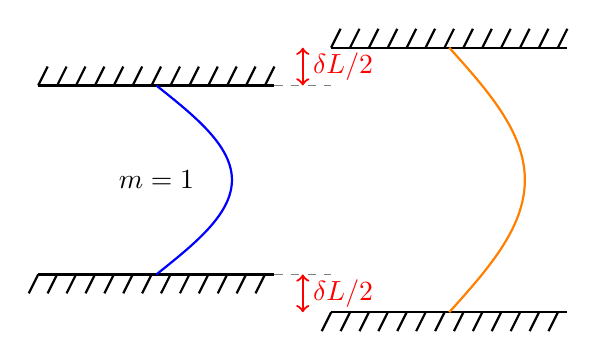
\begin{tikzpicture}[scale=1.2] % Scaled down slightly further
	
	% Parameters
	\def\L{2.0}
	\def\dL{0.4} % This is delta L / 2
	\def\gap{0.6} % Reduced gap between waveguides
	
	% -----------------------------
	% Left Waveguide (Narrow)
	% -----------------------------
	% Walls
	\draw[thick] (0,0) -- (2.5,0);   
	\draw[thick] (0,\L) -- (2.5,\L);  
	
	% Hatching
	\foreach \x in {0,0.2,...,2.5} {
		\draw[thick] (\x-0.1,-0.2) -- ++(0.1,0.2);
		\draw[thick] (\x,\L) -- ++(0.1, 0.2);
	}
	
	% Mode 1
	\draw[blue, thick, smooth, samples=200, domain=0:\L] 
	plot ({1.25 + 0.8*sin(pi/\L*\x r)}, \x);
	\node at (1.25, \L/2) {$m=1$};
	
	% -----------------------------
	% Right Waveguide (Wide)
	% -----------------------------
	\def\startX{2.5 + \gap}
	\def\endX{\startX + 2.5}
	\def\midX{\startX + 1.25}
	
	% Walls
	\draw[thick] (\startX,-\dL) -- (\endX,-\dL);   
	\draw[thick] (\startX,\L+\dL) -- (\endX,\L+\dL);  
	
	% Hatching
	\foreach \x in {3.1,3.3,...,5.6} { % Adjusted range manually for \startX=3.1, \endX=5.6
		\draw[thick] (\x-0.1,-\dL-0.2) -- ++(0.1,0.2);
		\draw[thick] (\x,\L+\dL) -- ++(0.1, 0.2);
	}
	
	% Mode 1
	\draw[orange, thick, smooth, samples=200, domain=-\dL:\L+\dL] 
	plot ({\midX + 0.8*sin(pi/(\L+2*\dL)*(\x+\dL) r)}, \x);
	% node at \midX removed as requested
	
	% -----------------------------
	% Annotations for dL/2
	% -----------------------------
	\def\annotX{2.5 + \gap/2}
	\draw[<->, red, thick] (\annotX, 0) -- (\annotX, -\dL) node[midway, right] {$\delta L/2$};
	\draw[<->, red, thick] (\annotX, \L) -- (\annotX, \L+\dL) node[midway, right] {$\delta L/2$};
	
	% Helper dashed lines
	\draw[dashed, gray] (2.5,0) -- (\startX,0);
	\draw[dashed, gray] (2.5,\L) -- (\startX,\L);
	
\end{tikzpicture}

		\begin{equation*}
			T(L) = \frac{\left|\int_{-L/2}^{L/2}dz \cos(\frac{2\pi}{L}z)\cos(\frac{2\pi}{L+\delta L}z)\right|^2 }
			{\left[\int_{-L/2}^{L/2}dz \cos^2(\frac{2\pi}{L}z)\right]
			\left[\int_{-(L+\delta L)/2}^{(L+\delta L)/2}dz\cos^2(\frac{2\pi}{L+\delta L}z) \right]}
		\end{equation*}
	}
	
	\only<2>{
		\begin{equation*}
			\begin{split}
				T(L) &= \frac{L}{L+\delta L} \text{sinc}^2\left(\frac{\pi \delta L}{L}\right)\\
				&\approx 1 - \frac{|\delta L|}{L}
			\end{split}
		\end{equation*}
	}

\end{frame}